\PassOptionsToPackage{unicode=true}{hyperref} % options for packages loaded elsewhere
\PassOptionsToPackage{hyphens}{url}
%
\documentclass[]{book}
\usepackage{lmodern}
\usepackage{amssymb,amsmath}
\usepackage{ifxetex,ifluatex}
\usepackage{fixltx2e} % provides \textsubscript
\ifnum 0\ifxetex 1\fi\ifluatex 1\fi=0 % if pdftex
  \usepackage[T1]{fontenc}
  \usepackage[utf8]{inputenc}
  \usepackage{textcomp} % provides euro and other symbols
\else % if luatex or xelatex
  \usepackage{unicode-math}
  \defaultfontfeatures{Ligatures=TeX,Scale=MatchLowercase}
\fi
% use upquote if available, for straight quotes in verbatim environments
\IfFileExists{upquote.sty}{\usepackage{upquote}}{}
% use microtype if available
\IfFileExists{microtype.sty}{%
\usepackage[]{microtype}
\UseMicrotypeSet[protrusion]{basicmath} % disable protrusion for tt fonts
}{}
\IfFileExists{parskip.sty}{%
\usepackage{parskip}
}{% else
\setlength{\parindent}{0pt}
\setlength{\parskip}{6pt plus 2pt minus 1pt}
}
\usepackage{hyperref}
\hypersetup{
            pdftitle={MA 5124 Financial Time Series Analysis \& Forecasting},
            pdfauthor={Dr.~Priyanga D. Talagala},
            pdfborder={0 0 0},
            breaklinks=true}
\urlstyle{same}  % don't use monospace font for urls
\usepackage{color}
\usepackage{fancyvrb}
\newcommand{\VerbBar}{|}
\newcommand{\VERB}{\Verb[commandchars=\\\{\}]}
\DefineVerbatimEnvironment{Highlighting}{Verbatim}{commandchars=\\\{\}}
% Add ',fontsize=\small' for more characters per line
\usepackage{framed}
\definecolor{shadecolor}{RGB}{248,248,248}
\newenvironment{Shaded}{\begin{snugshade}}{\end{snugshade}}
\newcommand{\AlertTok}[1]{\textcolor[rgb]{0.94,0.16,0.16}{#1}}
\newcommand{\AnnotationTok}[1]{\textcolor[rgb]{0.56,0.35,0.01}{\textbf{\textit{#1}}}}
\newcommand{\AttributeTok}[1]{\textcolor[rgb]{0.77,0.63,0.00}{#1}}
\newcommand{\BaseNTok}[1]{\textcolor[rgb]{0.00,0.00,0.81}{#1}}
\newcommand{\BuiltInTok}[1]{#1}
\newcommand{\CharTok}[1]{\textcolor[rgb]{0.31,0.60,0.02}{#1}}
\newcommand{\CommentTok}[1]{\textcolor[rgb]{0.56,0.35,0.01}{\textit{#1}}}
\newcommand{\CommentVarTok}[1]{\textcolor[rgb]{0.56,0.35,0.01}{\textbf{\textit{#1}}}}
\newcommand{\ConstantTok}[1]{\textcolor[rgb]{0.00,0.00,0.00}{#1}}
\newcommand{\ControlFlowTok}[1]{\textcolor[rgb]{0.13,0.29,0.53}{\textbf{#1}}}
\newcommand{\DataTypeTok}[1]{\textcolor[rgb]{0.13,0.29,0.53}{#1}}
\newcommand{\DecValTok}[1]{\textcolor[rgb]{0.00,0.00,0.81}{#1}}
\newcommand{\DocumentationTok}[1]{\textcolor[rgb]{0.56,0.35,0.01}{\textbf{\textit{#1}}}}
\newcommand{\ErrorTok}[1]{\textcolor[rgb]{0.64,0.00,0.00}{\textbf{#1}}}
\newcommand{\ExtensionTok}[1]{#1}
\newcommand{\FloatTok}[1]{\textcolor[rgb]{0.00,0.00,0.81}{#1}}
\newcommand{\FunctionTok}[1]{\textcolor[rgb]{0.00,0.00,0.00}{#1}}
\newcommand{\ImportTok}[1]{#1}
\newcommand{\InformationTok}[1]{\textcolor[rgb]{0.56,0.35,0.01}{\textbf{\textit{#1}}}}
\newcommand{\KeywordTok}[1]{\textcolor[rgb]{0.13,0.29,0.53}{\textbf{#1}}}
\newcommand{\NormalTok}[1]{#1}
\newcommand{\OperatorTok}[1]{\textcolor[rgb]{0.81,0.36,0.00}{\textbf{#1}}}
\newcommand{\OtherTok}[1]{\textcolor[rgb]{0.56,0.35,0.01}{#1}}
\newcommand{\PreprocessorTok}[1]{\textcolor[rgb]{0.56,0.35,0.01}{\textit{#1}}}
\newcommand{\RegionMarkerTok}[1]{#1}
\newcommand{\SpecialCharTok}[1]{\textcolor[rgb]{0.00,0.00,0.00}{#1}}
\newcommand{\SpecialStringTok}[1]{\textcolor[rgb]{0.31,0.60,0.02}{#1}}
\newcommand{\StringTok}[1]{\textcolor[rgb]{0.31,0.60,0.02}{#1}}
\newcommand{\VariableTok}[1]{\textcolor[rgb]{0.00,0.00,0.00}{#1}}
\newcommand{\VerbatimStringTok}[1]{\textcolor[rgb]{0.31,0.60,0.02}{#1}}
\newcommand{\WarningTok}[1]{\textcolor[rgb]{0.56,0.35,0.01}{\textbf{\textit{#1}}}}
\usepackage{longtable,booktabs}
% Fix footnotes in tables (requires footnote package)
\IfFileExists{footnote.sty}{\usepackage{footnote}\makesavenoteenv{longtable}}{}
\usepackage{graphicx,grffile}
\makeatletter
\def\maxwidth{\ifdim\Gin@nat@width>\linewidth\linewidth\else\Gin@nat@width\fi}
\def\maxheight{\ifdim\Gin@nat@height>\textheight\textheight\else\Gin@nat@height\fi}
\makeatother
% Scale images if necessary, so that they will not overflow the page
% margins by default, and it is still possible to overwrite the defaults
% using explicit options in \includegraphics[width, height, ...]{}
\setkeys{Gin}{width=\maxwidth,height=\maxheight,keepaspectratio}
\setlength{\emergencystretch}{3em}  % prevent overfull lines
\providecommand{\tightlist}{%
  \setlength{\itemsep}{0pt}\setlength{\parskip}{0pt}}
\setcounter{secnumdepth}{5}
% Redefines (sub)paragraphs to behave more like sections
\ifx\paragraph\undefined\else
\let\oldparagraph\paragraph
\renewcommand{\paragraph}[1]{\oldparagraph{#1}\mbox{}}
\fi
\ifx\subparagraph\undefined\else
\let\oldsubparagraph\subparagraph
\renewcommand{\subparagraph}[1]{\oldsubparagraph{#1}\mbox{}}
\fi

% set default figure placement to htbp
\makeatletter
\def\fps@figure{htbp}
\makeatother

\usepackage{booktabs}
\usepackage{amsthm}
\makeatletter
\def\thm@space@setup{%
  \thm@preskip=8pt plus 2pt minus 4pt
  \thm@postskip=\thm@preskip
}
\makeatother
\usepackage[]{natbib}
\bibliographystyle{apalike}

\title{MA 5124 Financial Time Series Analysis \& Forecasting}
\author{Dr.~Priyanga D. Talagala}
\date{2021-01-10}

\begin{document}
\maketitle

{
\setcounter{tocdepth}{1}
\tableofcontents
}
\hypertarget{course-syllabus}{%
\chapter*{Course Syllabus}\label{course-syllabus}}
\addcontentsline{toc}{chapter}{Course Syllabus}

\pagenumbering{arabic}

\textbf{Module Code:} MA 5124

\textbf{Title:} Financial Time Series Analysis \& Forecasting

\textbf{Credits:} 4

\hypertarget{pre-requiites}{%
\section*{Pre-requiites}\label{pre-requiites}}
\addcontentsline{toc}{section}{Pre-requiites}

None

\hypertarget{learning-objectives}{%
\section*{Learning Objectives}\label{learning-objectives}}
\addcontentsline{toc}{section}{Learning Objectives}

\begin{itemize}
\tightlist
\item
  The purpose of this course is to provide students with introductory tools for the time series analysis of financial time series.
\item
  Analyze of data series based on stochastic and non stochastic models
\end{itemize}

\hypertarget{learning-outcomes}{%
\section*{Learning Outcomes}\label{learning-outcomes}}
\addcontentsline{toc}{section}{Learning Outcomes}

\begin{itemize}
\tightlist
\item
  On successful completion of this course, students will be able to provide more than an introductory treatment of the topics.
\item
  Students are encouraged to pursue further study in this area if they find that the topics covered in this course.
\end{itemize}

\hypertarget{outline-syllabus}{%
\section*{Outline Syllabus}\label{outline-syllabus}}
\addcontentsline{toc}{section}{Outline Syllabus}

\begin{itemize}
\tightlist
\item
  Definition and examples of time series
\item
  back-shift and differencing-operators, - strong and weak stationarity, definition of ACF, PACF.
\item
  Definitions and properties of the \(MA(q), MA(\infty), AR(p), AR(\infty)\)
  and \(ARMA(p,q)\),in particualr their acf's
\item
  causal stationarity of AR
\item
  invertibility of MA models and causal stationarity and invertibility of ARMA; - concept of spectral density function and its applications
\item
  definition and properties of integrated \(ARIMA(p,d,q)\) processes
\item
  definition and properties of random walks with or without drift.
\item
  Model selection following the AIC and BIC
\item
  brief introduction to linear prediction and calculation of forecasting intervals for normal ARMA models
\item
  point and interval forecasts for normal random walks with or without drift.
\item
  Definition and properties of the VAR (vector autoregressive) model, arrange a univariate time series as a multivariate Markov model.
\item
  Nonlinear properties of financial time series
\item
  definition and properties of the well known ARCH, GARCH etc.
\item
  Cointegration in Single Equations, Modeling and Forecasting Financial Time Series.
\end{itemize}

\hypertarget{method-of-assessment}{%
\section*{Method of Assessment}\label{method-of-assessment}}
\addcontentsline{toc}{section}{Method of Assessment}

\begin{itemize}
\tightlist
\item
  Assignment 30\%
\item
  End-semester examination 70\%
\end{itemize}

\hypertarget{lecturer}{%
\section*{Lecturer}\label{lecturer}}
\addcontentsline{toc}{section}{Lecturer}

Dr.~Priyanga D. Talagala

\hypertarget{schedule}{%
\section*{Schedule}\label{schedule}}
\addcontentsline{toc}{section}{Schedule}

Lectures:

\begin{itemize}
\tightlist
\item
  Sunday {[}9.00am -12.00 noon{]}
\end{itemize}

\hypertarget{copyright-notice}{%
\section*{Copyright Notice}\label{copyright-notice}}
\addcontentsline{toc}{section}{Copyright Notice}

My lectures and course materials, including presentations, tests, exams, outlines, and similar materials, are protected by copyright. I am the exclusive owner of copyright in those materials I create. I encourage you to take notes and make copies of course materials for your own educational use. However, you may not, nor may you knowingly allow others to reproduce or distribute lecture notes and course materials publicly without my express written consent.

\hypertarget{intro}{%
\chapter{Intordution to Time Series Forecasting}\label{intro}}

\hypertarget{arima-models}{%
\chapter{ARIMA models}\label{arima-models}}

\begin{itemize}
\tightlist
\item
  \textbf{AR}: autoregressive (lagged observations as inputs)
\item
  \textbf{I}: integrated (differencing to make series stationary)
\item
  \textbf{MA}: moving average (lagged errors as inputs)
\end{itemize}

An ARIMA model is rarely interpretable in terms of visible data structures like trend and seasonality. But it can capture a huge range of time series patterns.

\hypertarget{stationarity-and-differencing}{%
\section{Stationarity and differencing}\label{stationarity-and-differencing}}

\hypertarget{stationarity}{%
\subsection{Stationarity}\label{stationarity}}

\textbf{Definition}

If \(\{y_t\}\) is a stationary time series, then for all \(s\), the distribution of \((y_t,\dots,y_{t+s})\) does not depend on \(t\).

A \textbf{stationary series} is:

\begin{itemize}
\item
  roughly horizontal
\item
  constant variance
\item
  no patterns predictable in the long-term
\item
  Transformations help to stabilize the variance.
\item
  For ARIMA modelling, we also need to stabilize the mean.
\end{itemize}

\textbf{Identifying non-stationary series}

\begin{itemize}
\tightlist
\item
  time plot.
\item
  The ACF of stationary data drops to zero relatively quickly
\item
  The ACF of non-stationary data decreases slowly.
\item
  For non-stationary data, the value of r1 is often large and positive.
\end{itemize}

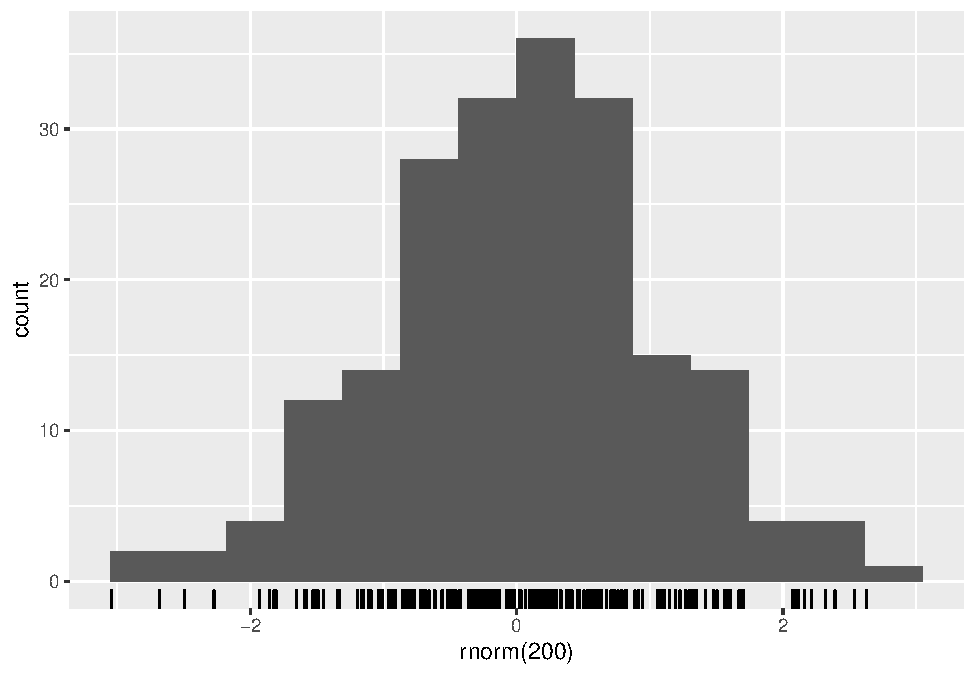
\includegraphics{bookdown-demo_files/figure-latex/unnamed-chunk-1-1.pdf}

\hypertarget{differencing}{%
\subsection{Differencing}\label{differencing}}

\begin{itemize}
\tightlist
\item
  Differencing helps to \textbf{stabilize the mean}.
\item
  The differenced series is the \emph{change} between each observation in the original series: \(y'_t = y_t - y_{t-1}\).
\item
  The differenced series will have only \(T-1\) values since it is not possible to calculate a difference \(y_1'\) for the first observation.
\end{itemize}

\hypertarget{second-order-differencing}{%
\subsection{Second-order differencing}\label{second-order-differencing}}

Occasionally the differenced data will not appear stationary and it may be necessary to difference the data a second time:

\[y''_{t} = y'_{t} - y'_{t - 1}\]
\[= (y_t - y_{t-1}) - (y_{t-1}-y_{t-2})\]
\[= y_t - 2y_{t-1} +y_{t-2}.\]

\begin{itemize}
\tightlist
\item
  \(y_t''\) will have \(T-2\) values.
\item
  In practice, it is almost never necessary to go beyond second-order differences.
\end{itemize}

\hypertarget{seasonal-differencing}{%
\subsection{Seasonal differencing}\label{seasonal-differencing}}

A seasonal difference is the difference between an observation and the corresponding observation from the previous year.

\[y'_t = y_t - y_{t-m}\]

where \(m=\) number of seasons.

\begin{itemize}
\tightlist
\item
  For monthly data \(m=12\).
\item
  For quarterly data \(m=4\).
\end{itemize}

\textbf{Example : Electricity production}

\begin{Shaded}
\begin{Highlighting}[]
\NormalTok{usmelec }\OperatorTok\StringTok{ }\KeywordTok{autoplot}\NormalTok{( Generation}
\NormalTok{)}
\end{Highlighting}
\end{Shaded}

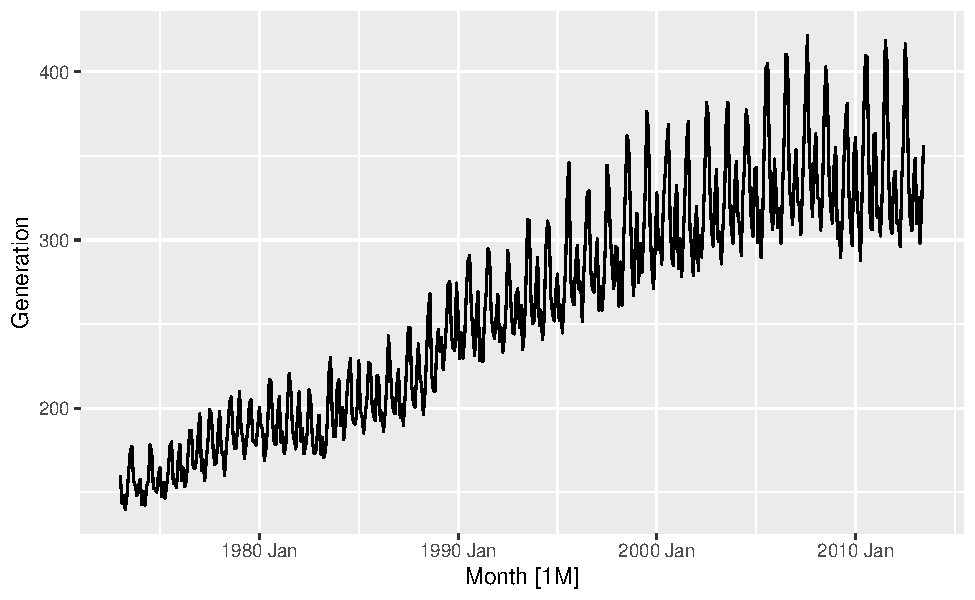
\includegraphics{bookdown-demo_files/figure-latex/unnamed-chunk-3-1.pdf}

\begin{Shaded}
\begin{Highlighting}[]
\NormalTok{usmelec }\OperatorTok\StringTok{ }\KeywordTok{autoplot}\NormalTok{( }\KeywordTok{log}\NormalTok{(Generation)}
\NormalTok{)}
\end{Highlighting}
\end{Shaded}

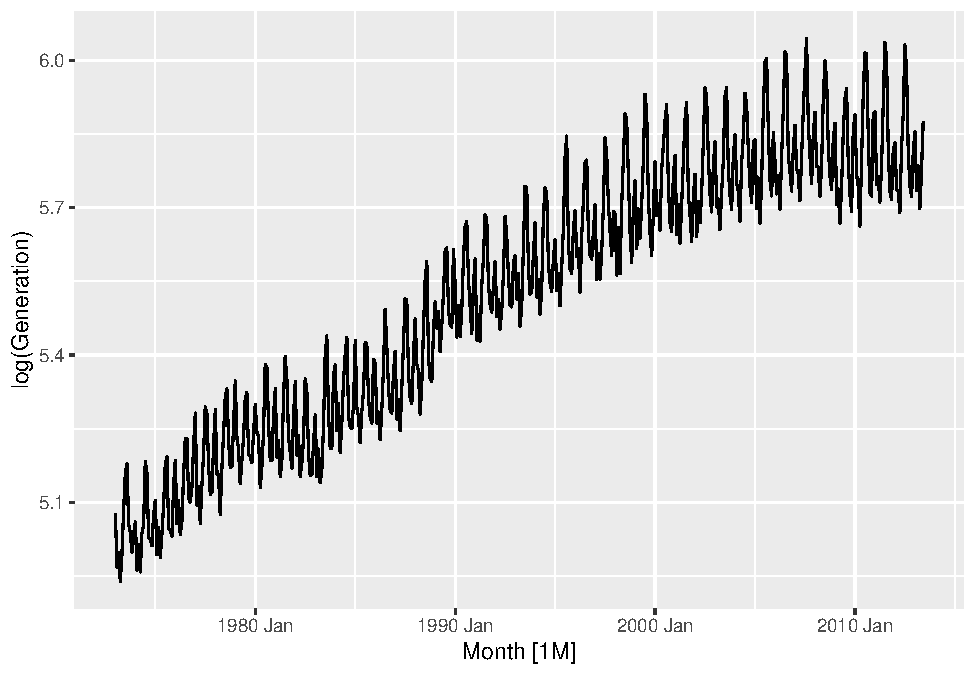
\includegraphics{bookdown-demo_files/figure-latex/unnamed-chunk-4-1.pdf}

\begin{Shaded}
\begin{Highlighting}[]
\NormalTok{usmelec }\OperatorTok\StringTok{ }\KeywordTok{autoplot}\NormalTok{( }\KeywordTok{log}\NormalTok{(Generation) }\OperatorTok\StringTok{ }\KeywordTok{difference}\NormalTok{(}\DecValTok{12}\NormalTok{)}
\NormalTok{) }
\end{Highlighting}
\end{Shaded}

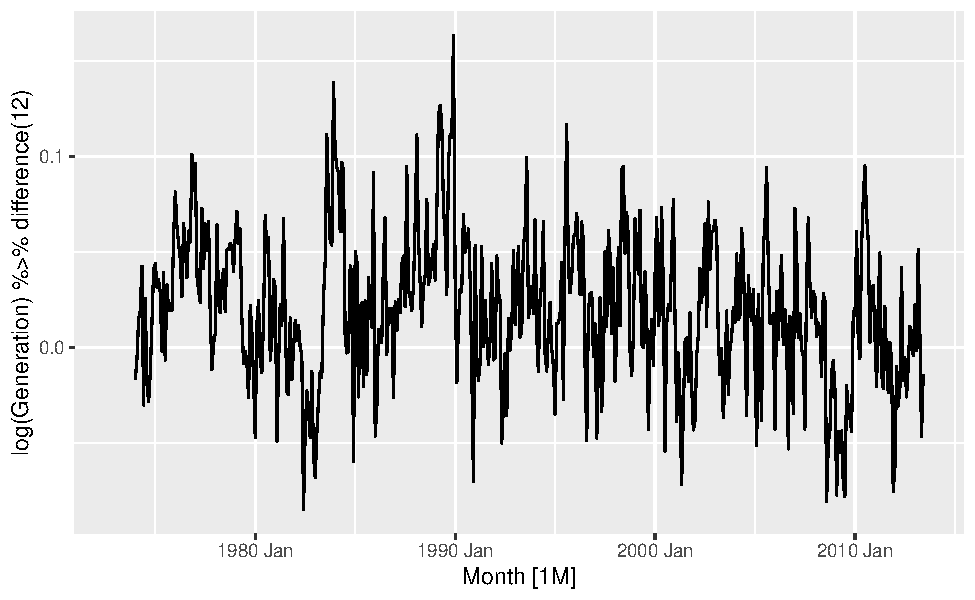
\includegraphics{bookdown-demo_files/figure-latex/unnamed-chunk-5-1.pdf}

\begin{Shaded}
\begin{Highlighting}[]
\NormalTok{ usmelec }\OperatorTok\StringTok{ }\KeywordTok{autoplot}\NormalTok{(}
\KeywordTok{log}\NormalTok{(Generation) }\OperatorTok\StringTok{ }\KeywordTok{difference}\NormalTok{(}\DecValTok{12}\NormalTok{) }\OperatorTok\StringTok{ }\KeywordTok{difference}\NormalTok{()}
\NormalTok{)}
\end{Highlighting}
\end{Shaded}

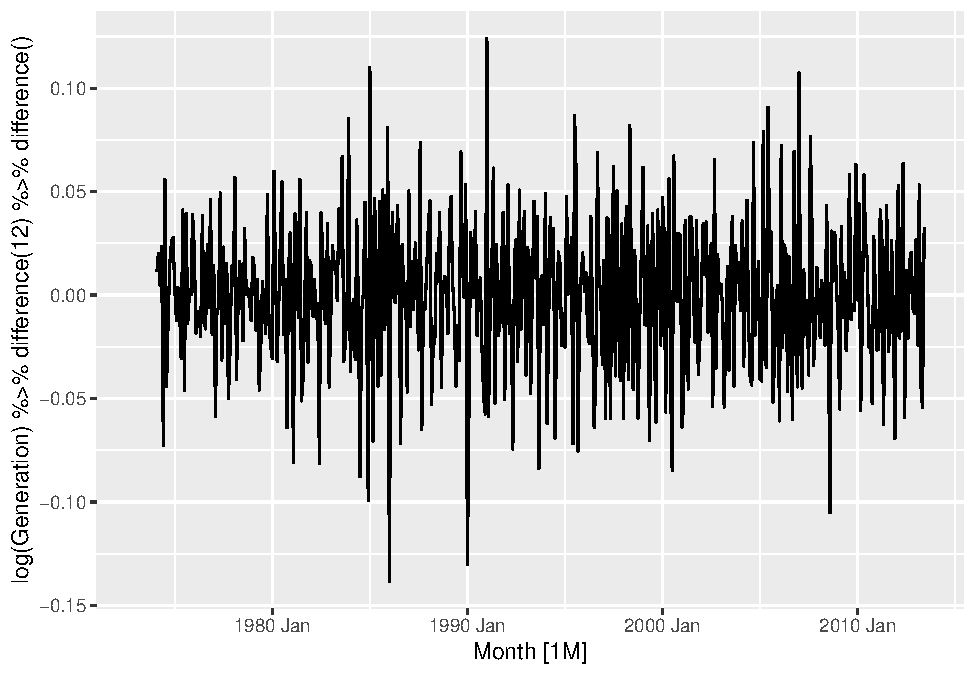
\includegraphics{bookdown-demo_files/figure-latex/unnamed-chunk-6-1.pdf}

\begin{itemize}
\tightlist
\item
  Seasonally differenced series is closer to being stationary.
\item
  Remaining non-stationarity can be removed with further first difference.
\end{itemize}

If \(y'_t = y_t - y_{t-12}\) denotes seasonally differenced series, then twice-differenced series is

\[y^*_t = y'_t - y'_{t-1}\]
\[= (y_t - y_{t-12}) - (y_{t-1} - y_{t-13})\]
\[= y_t - y_{t-1} - y_{t-12} + y_{t-13}.\]

When both seasonal and first differences are applied \(\dots\)
- it makes no difference which is done first---the result will be the same.
- If seasonality is strong, we recommend that seasonal differencing be done first because sometimes the resulting series will be stationary and there will be no need for further first difference.

It is important that if differencing is used, the differences are interpretable.

\hypertarget{interpretation-of-differencing}{%
\subsection{Interpretation of differencing}\label{interpretation-of-differencing}}

\begin{itemize}
\tightlist
\item
  first differences are the change between one observation and the next;
\item
  seasonal differences are the change between one year to the next.
\end{itemize}

But taking lag 3 differences for yearly data, for example, results in a model which cannot be sensibly interpreted.

\hypertarget{exponential-smoothing}{%
\chapter{Exponential Smoothing}\label{exponential-smoothing}}

\bibliography{book.bib,packages.bib}

\end{document}
